% @Author: Taha Bouhsine


%%%%%%%%%%%%%%%%%%%%%%%%%%%%
% CHAPTER                  %
%%%%%%%%%%%%%%%%%%%%%%%%%%%%
\setcounter{mtc}{9}

\chapter{Technical and environmental study}%
\label{chap:chapter_tree}
\minitoc
\section{Capture of technical needs}
The capture of technical needs identifies all the constraints and the choices dimensioning the design of the system.

The tools and materials selected as well as the management of integration constraints generally conditioning the prerequisites of general architecture.

The capture of technical needs is as follows:
\begin{itemize}\addtolength{\itemsep}{-0.35\baselineskip}
      \item
            Capturing software specifications.

      \item
            Capturing specifications related to hardware configuration.

\end{itemize}

\subsection{Capturing software specifications}
Once the hardware specifications have been determined, we move on to the non-functional specifications, in other words, technical or software specifications.

These are technical features that the system will provide to the user regardless of the business or functional term.

We will, therefore, list a list of technical functionalities that our system will be able to provide and offer to users, which is why we have introduced the concepts of operator and technical use cases:

\paragraph{Technical actors}
Also called "technical actors" of the system, these are the actors who benefit from the technical functionalities of the system:
\begin{itemize}\addtolength{\itemsep}{-0.35\baselineskip}
      \item
            User: These are the people who use the system functionality in one way or another.
      \item
            Administrator: this is the person responsible for managing all the management of the platform as well as that of the users.
\end{itemize}

\paragraph{Identification of technical use cases}

\begin{longtable}{|m{10em}|m{10em}|m{10em}|}\hline
      \multirow{4}{*}{Security management} & \multirow{5}{*}{Authentication}          & UC1-Register                                                    \\\cline{3-3}
                                           &                                          & UC2-Login                                                       \\\cline{3-3}
                                           &                                          & UC3-Reset Password                                              \\\cline{3-3}
                                           &                                          & UC4-Change password                                             \\\cline{3-3}
                                           &                                          & UC5-Logout                                                      \\\cline{2-3}
                                           & \multirow{1}{*}{Confidentiality}         & UC6-Role management                                             \\\cline{2-3}
                                           & \multirow{2}{*}{Secure payment}          & UC7-Send Payment                                                \\\cline{3-3}
                                           &                                          & UC8-Receive Payment                                             \\\cline{2-3}
                                           & \multirow{2}{*}{Backup and restore}      & UC9-Save the database                                           \\\cline{3-3}
                                           &                                          & UC10-Restore the database                                       \\\hline
      \multirow{7}{*}{Data managment}      & \multirow{1}{*}{Dynamic data}            & UC11-Dynamic data dispaly                                       \\\cline{2-3}
                                           & \multirow{1}{*}{Integrity}               & UC12-Simultaneous updates                                       \\\cline{2-3}
                                           & \multirow{1}{*}{Interoperability}        & UC13-Network deployment                                         \\\cline{2-3}
                                           & \multirow{1}{*}{Compatibility}           & UC14-Run on different browsers and platforms                    \\\cline{2-3}
                                           & \multirow{2}{*}{History}                 & UC15-Get all the user created projects fundraised               \\\cline{3-3}
                                           &                                          & UC16-Get all the user created projects fundraised               \\\cline{2-3}
                                           & \multirow{1}{*}{Statistics}              & UC17-Display platform statistics                                \\\cline{2-3}
                                           & \multirow{1}{*}{Fund}                    & UC18-Fund migration from anonymous user                         \\\hline
      \multirow{4}{*}{Help management}     & \multirow{2}{*}{Gestion des erreurs}     & UC19-Logging Viewing types of errors                            \\\cline{3-3}
                                           &                                          & UC20-Send the error by email to the administrator               \\\cline{2-3}
                                           & \multirow{1}{*}{Aide en ligne}           & UC21-Consult the user help Guide                                \\\cline{2-3}
                                           & \multirow{1}{*}{Notifications}           & UC22-Confirmation or error message                              \\\cline{2-3}
                                           & \multirow{1}{*}{Mails}                   & UC23-Sending emails                                             \\\hline
      \multirow{2}{*}{Payment management}  & \multirow{1}{*}{Multi-currency platform} & UC24-Choose a currency for purchase and payment                 \\\cline{2-3}
                                           & \multirow{1}{*}{Payment method}          & UC25-Possibility to choose a payment method                     \\\hline
      \multirow{3}{*}{Optimization}        & \multirow{1}{*}{Navigation}              & UC26-Nested operations                                          \\\cline{2-3}
                                           & \multirow{1}{*}{Sharing}                 & UC27-Possibility to share your donation                         \\\cline{2-3}
                                           & \multirow{1}{*}{Theming}                 & UC28-Possibility to switch themes between dark and light themes \\\hline

      \caption{Identification of technical objectives and use cases}
      \label{tab:id_tech_objec_uc}
\end{longtable}

\paragraph{ Technical description use cases }
View all the use cases described in the appendix \ref{sec:ucd}


\subsection{Capturing hardware specifications}

\begin{figure}[!ht]
      \centering
      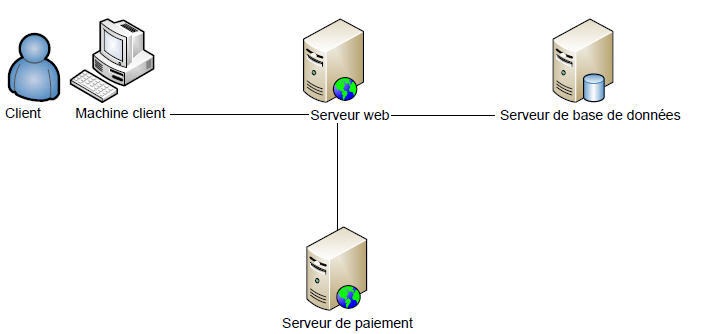
\includegraphics[scale=0.60]{assets/network-arch.jpg}
      \caption{Sahem Platform Actors}
      \label{fig:sahemactors}
\end{figure}

\section{Adopted Architecture}

\subsection{Model View Controller Design Pattern}

The Model View Controller (MVC) design pattern specifies that an application consists of a data model, presentation information, and control information. The pattern requires that each of these be separated into different objects.

MVC is more of an architectural pattern, but not for a complete application. MVC mostly relates to the UI / interaction layer of an application. We’re still going to need a business logic layer, maybe some service layer and data access layer.
\begin{enumerate}
      \item Model contains only the pure application data, it contains no logic describing how to present the data to a user.
      \item View presents the model’s data to the user. The view knows how to access the model’s data, but it does not know what this data means or what the user can do to manipulate it.
      \item Controller exists between the view and the model. It listens to events triggered by the view (or another external source) and executes the appropriate reaction to these events. In most cases, the reaction is to call a method on the model. Since the view and the model are connected through a notification mechanism, the result of this action is then automatically reflected in the view.
\end{enumerate}

\begin{figure}[!ht]
      \center
      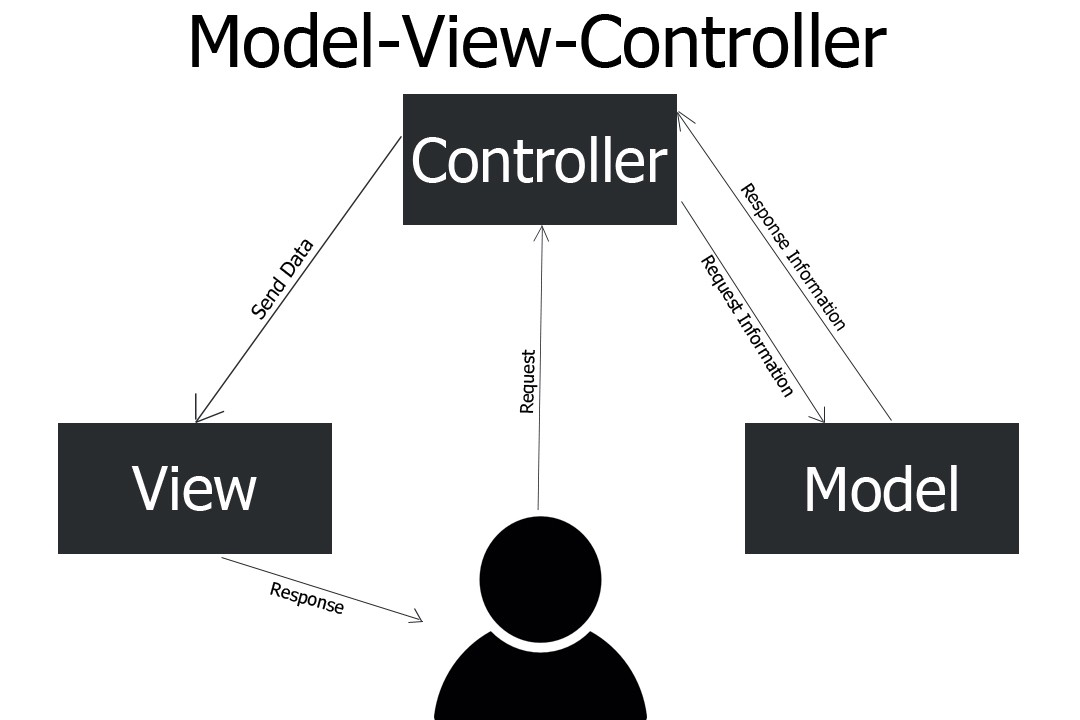
\includegraphics[scale=0.30]{assets/mvc.jpg}
      \caption{Model View Controller}
      \label{fig:mvc}
\end{figure}
% %%%%%%%
\subsection{Representational State Transfer Architecture}
REST, or REpresentational State Transfer, is an architectural style for providing standards between computer systems on the web, making it easier for systems to communicate with each other. REST-compliant systems, often called RESTful systems, are characterized by how they are stateless and separate the concerns of client and server. We will go into what these terms mean and why they are beneficial characteristics for services on the Web.
%%%%
\subsection{Software as a Service}
Software as a Service or SaaS , which allows us to set up services, such as application servers and databases, as needed to create the apps we need. This type of system typically works in a cloud or hybrid cloud environment, which often makes provisioning of servers and software as simple as entering some configurations and clicking a button.

This type of setup is perfect for the MEAN stack, as each piece of the MEAN stack is easily placed into the cloud and thus can be easily provisioned, so they are widely available on SaaS services and can be used quickly when needed. If we are looking for a good development stack, the MEAN stack has much to offer for IT management as well as for developers!
%%%%

\subsection{Monolithic Applications}

If all the functionalities of a project exist in a single codebase, then that application is known as a monolithic application. We all must have designed a monolithic application in our lives in which we were given a problem statement and were asked to design a system with various functionalities. We design our application in various layers like presentation, service, and persistence and then deploy that codebase as a single jar/war file. This is nothing but a monolithic application where “mono” represents the single codebase containing all the required functionalities.
\begin{figure}[!ht]
      \center
      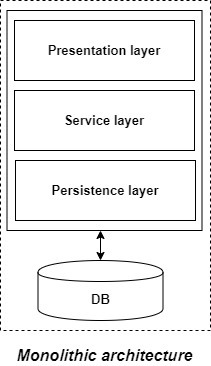
\includegraphics[scale=0.60]{assets/monolithic.jpg}
      \caption{Monolithic Applications}
      \label{fig:monoapp}
\end{figure}

Disadvantages of Monolithic applications:
\begin{enumerate}
      \item
            It becomes too large with time and hence, difficult to manage.
      \item
            We need to redeploy the whole application even for a small change.
      \item
            As the size of the application increases, its start-up and deployment time also increases.
      \item
            For any new developer joining the project, it is very difficult to understand the logic of a large Monolithic application even if his responsibility is related to a single functionality.
      \item
            Even if a single part of the application is facing a large load/traffic, we need to deploy the instances of the whole application in multiple servers. It is very inefficient and takes up more resources unnecessarily. Hence, horizontal scaling is not feasible in monolithic applications.
      \item
            It is very difficult to adopt any new technology which is well suited for a particular functionality as it affects the whole application, both in terms of time and cost.
      \item
            It is not very reliable as a single bug in any module can bring down the whole monolithic application.
\end{enumerate}
Advantages of monolithic applications:
\begin{enumerate}
      \item
            Simple to develop relative to microservices where skilled developers are required in order to identify and develop the services.
      \item
            Easier to deploy as only a single jar/war file is deployed.
      \item
            Relatively easier and simple to develop in comparison to microservices architecture.
      \item
            The problems of network latency and security are relatively less in comparison to microservices architecture.
\end{enumerate}

%%%





